\documentclass{article}
\usepackage[utf8]{inputenc}
\usepackage[english]{babel}
\usepackage{apacite}
\usepackage{graphicx}
\usepackage{mathptmx}
\usepackage[font = {small, it}]{caption}
\DeclareCaptionLabelFormat{cont}{#1~#2\alph{ContinuedFloat}}
\captionsetup[ContinuedFloat]{labelformat=cont}
%\usepackage{subcaption}
\usepackage{subfigure}
\usepackage{float}
\usepackage{fancyhdr}

\fancypagestyle{plain}{
\fancyhf{}
\rhead{Mikkel Werling, 201706722}
\lhead{PyCipio}
\cfoot{\thepage}
}
\pagestyle{plain}

\setlength{\parindent}{2em}
\setlength{\parskip}{1em}
\renewcommand{\baselinestretch}{1.5}

\title{PyCipio: Bayesian Time-series Prediction}
\author{Mikkel Werling\\201706722}
\date{27/05/2021}
\begin{document}
\maketitle
\section{Introduction}
\subsection{Time Series Forecasting}
\subsection{Decomposition of a Signal}

$$y(t) = g(t) + s(t) + \epsilon$$

$$y(t) = g(t) \cdot s(t) \cdot \epsilon $$

$$g(t) = \alpha + \beta \cdot x$$

$$s(t) = \sum _{n=1} ^N \left( a_n cos(\frac{2 \pi n t}{P}) + b_n sin(\frac{2 \pi n t}{P}) \right)$$

$$F(t) = \left[ cos(\frac{2 \pi 1 t}{7}), \dots, sin(\frac{2 \pi 8 t}{7}) \right]$$

$$s(t) = F(t) \cdot \omega$$

$$y(t) = alpha + beta \cdot x + s_1(t) + s_2(t)$$

\begin{figure}[ht]
    \centering
    \subfigure[First plot]{%
        \label{fig:supfigure1}
        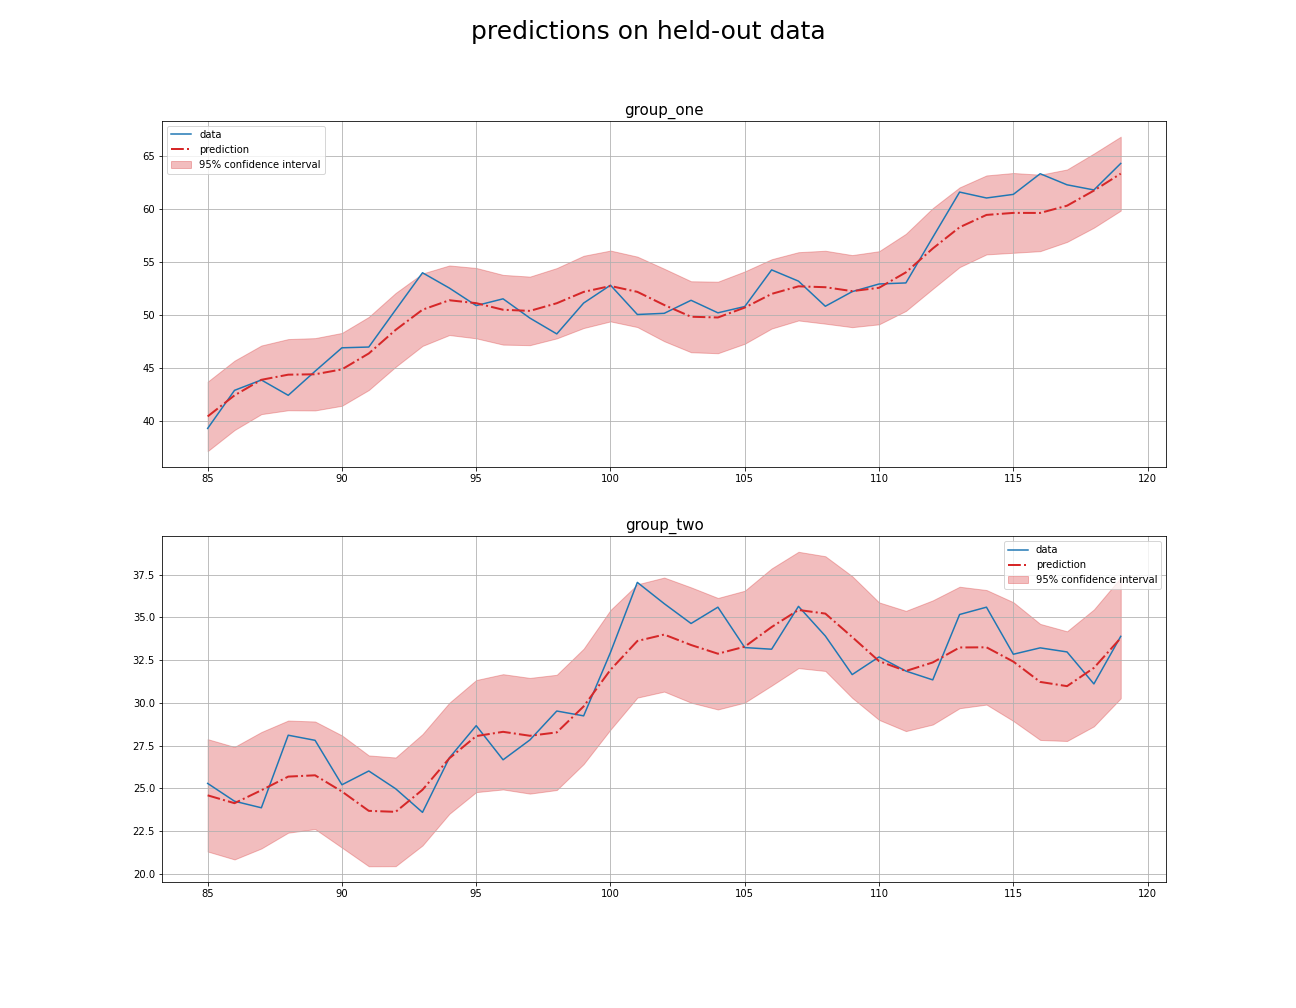
\includegraphics[width = 0.30 \textwidth]{../plots/ex1_first_plot_predict_idx_all}}
    \quad
    \subfigure[Second plot]{%
        \label{fig:supfigure2}
        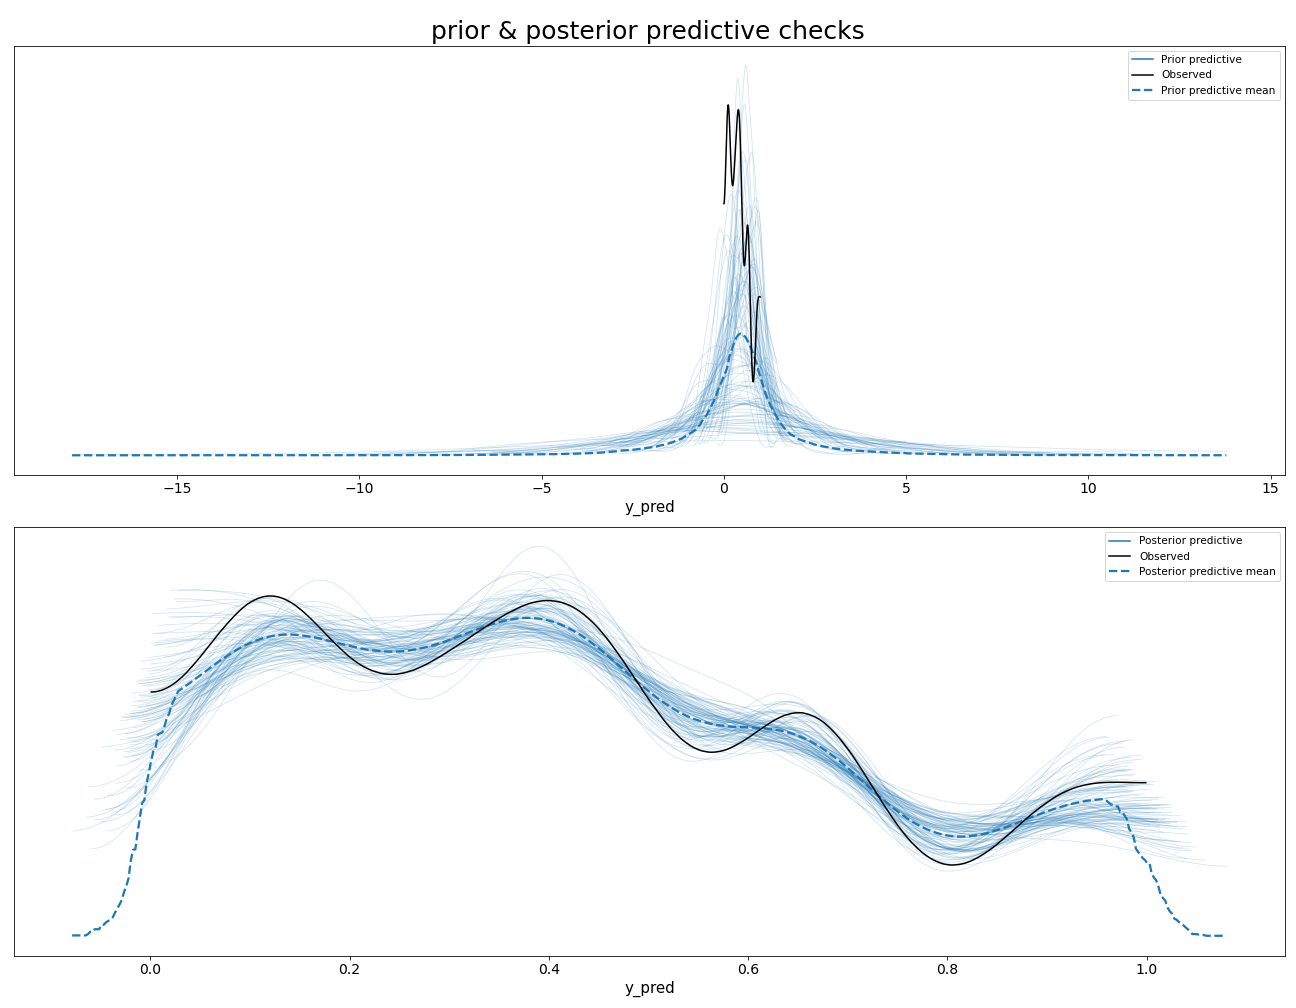
\includegraphics[width = 0.30 \textwidth]{../plots/ex1_first_plot_pp.png}}
    \subfigure[Third Plot]{%
        \label{fig:supfigure3}
        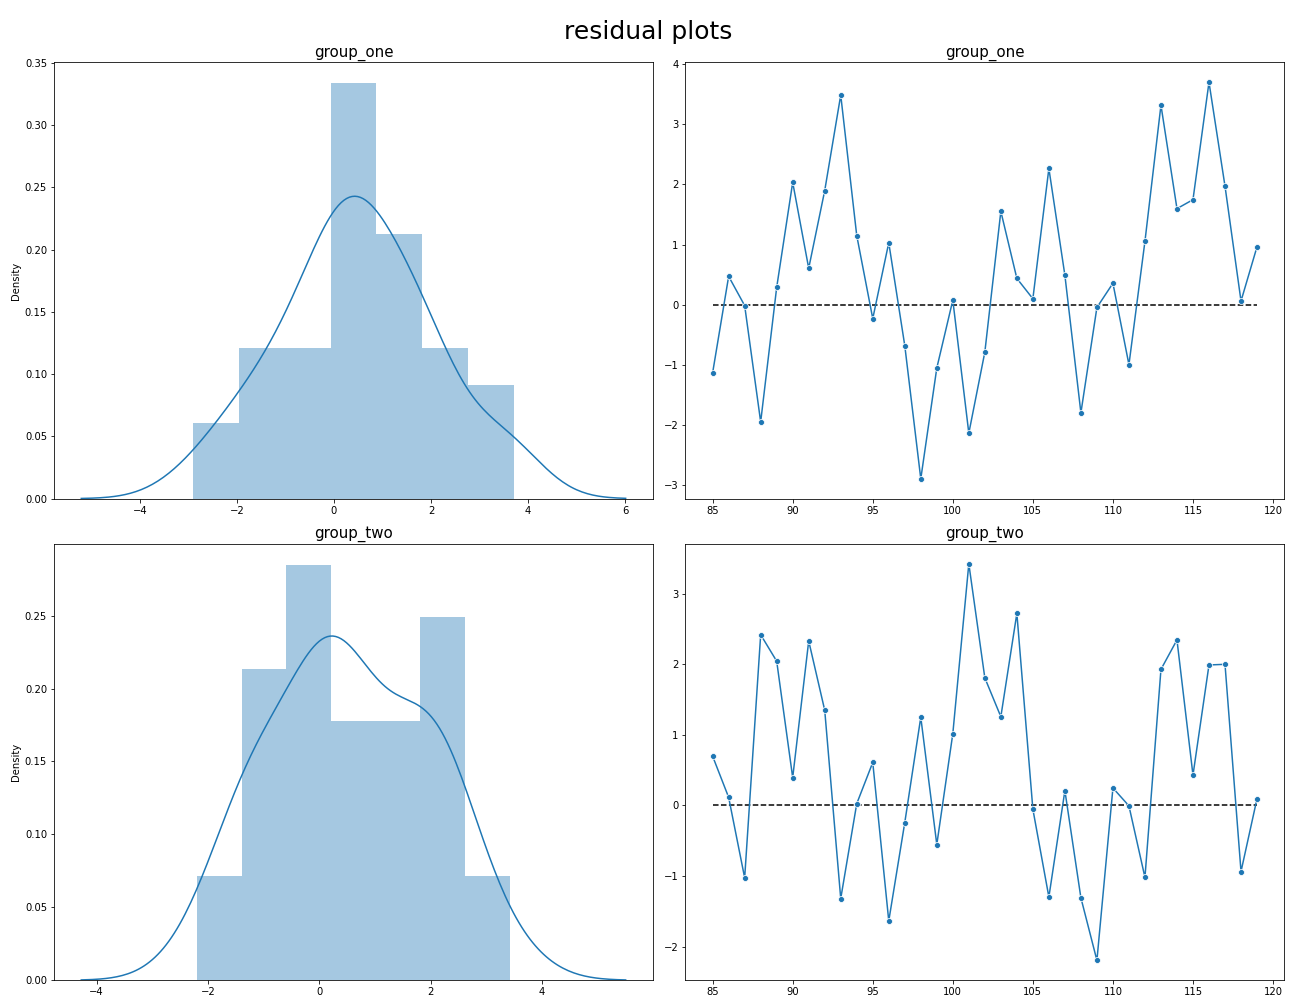
\includegraphics[width = 0.30 \textwidth]{../plots/ex1_first_residual_plots_all.png}}
    \quad
    \subfigure[Fourth plot]{%
        \label{fig:supfigure4}
        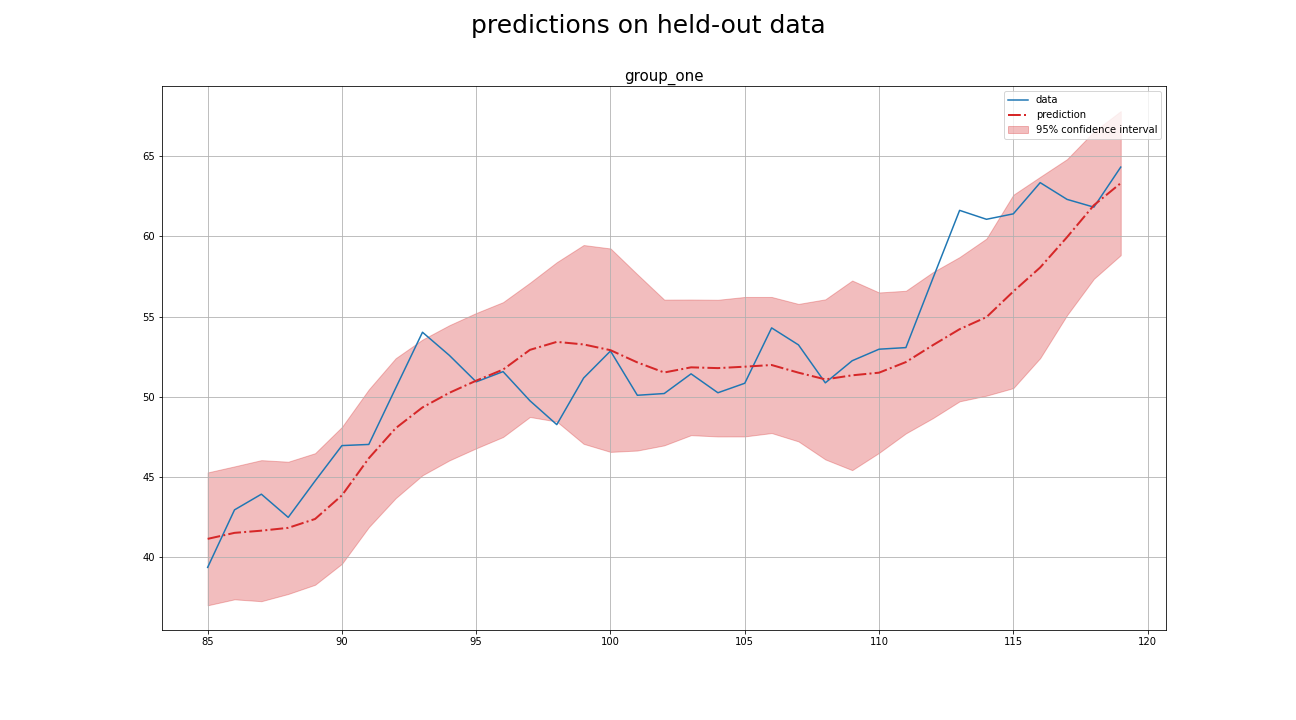
\includegraphics[width = 0.45 \textwidth]{../plots/ex1_second_plot_predict_idx_single.png}}
    
    \caption{Predictions in one and 2 groups}
\end{figure}


%\bibliographystyle{apacite}

%\bibliography{cite2}

\end{document}